\begin{center}
	\begin{tikzpicture}[x=1cm,y=1cm]
	%\pgfresetboundingbox
	\draw[use as bounding box, anchor = north west,draw=gray] (-5.5,-3.25) rectangle (5.5,3.25);
	\clip (-5.5,-3.25) rectangle (5.5,3.25);
	\node[anchor =north west] (text) at (-5.25,3.25){\begin{minipage}{10.0cm}
	Warning: this talk contains some \textit{light} mathematics
	\end{minipage}};
	\visible<1->{\node[anchor=west] (figure) at (-5.5,-1.5){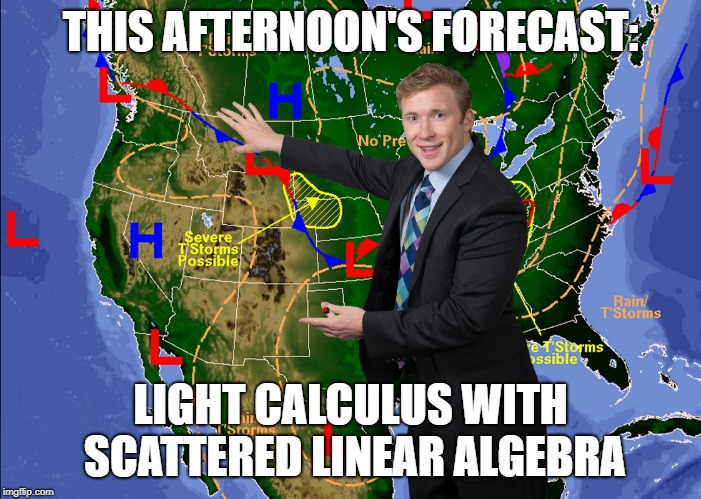
\includegraphics[width=3.5cm]{images-top/weather.jpg}};}
\end{tikzpicture}
\end{center}
